% Review uses a separate float page. Place these two pairs near their
% discussion when integrating with the full manuscript.
\begin{figure}[p]
  \centering
  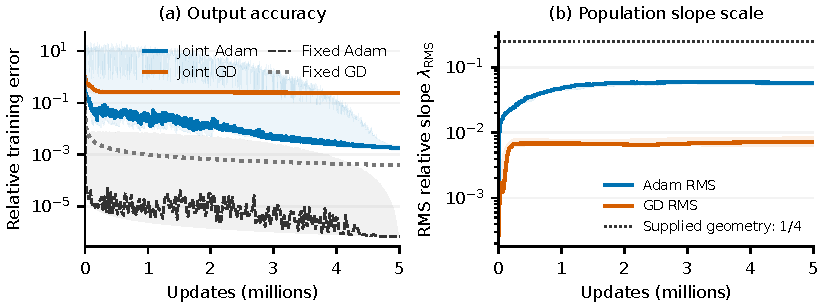
\includegraphics[width=\linewidth]{results/checkpoint_D_optimizers/expD34_readout_race/population_output/evidence/paper_latex_figures/joint_acquisition_rms.pdf}
  \caption{\textbf{Limited scale acquisition accompanies the precision gap.}
  Mixed sine, width 512, five paired seeds, five million full-batch updates.
  Left: relative training errors with trained readouts; fixed Adam/GD use
  uniform $\lambda=1/4$ features. Right: RMS relative slopes, $h=2/467$.
  Bands retain seed variation and within-bin extrema. Joint and fixed-Adam
  recipes use final-validation selection (Appendix~\ref{app:scale-experiments}).}
  \label{fig:scale-observation}
\end{figure}

\begin{figure}[p]
  \centering
  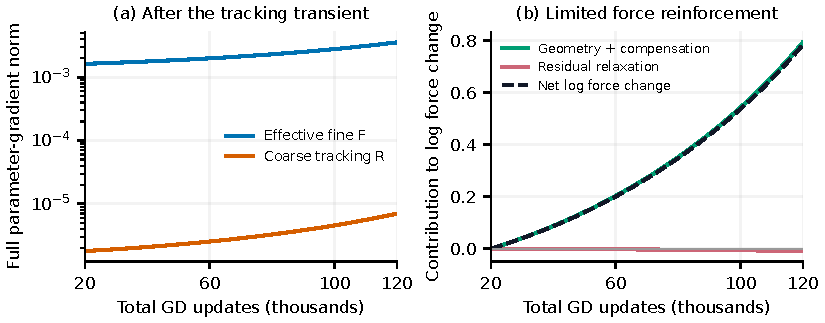
\includegraphics[width=\linewidth]{results/checkpoint_D_optimizers/expD34_readout_race/population_output/evidence/paper_latex_figures/tracking_and_reinforcement.pdf}
  \caption{\textbf{Weak effective force survives positive reinforcement.}
  Matched smooth-step continuations, width 705, from age 20k to 120k.
  Left: GD full-parameter gradient norms; tracking stays below 0.2\% of
  effective force at saved times. Right: cumulative terms
  in~\eqref{eq:scale-force-identity} along paired effective flow.
  Both axes use total GD updates with $\eta=0.002$; paired force norms
  differ by less than 0.08\%.}
  \label{fig:scale-mechanism}
\end{figure}
